\chapter{Πειραματική Διαδικασία}
\label{chap:5}
\thispagestyle{plain}
Η εκπαίδευση του νευρωνικού έγινε σε μονάδα επεξεργασίας γραφικών NVIDIA GEFORCE RTX 2080 με 8GB μνήμη και έκδοση CUDA 10.1. Επιπλέον, έγινε χρήση Python version 2.7, Τensorflow version 1.13 και Κeras version 2.2.4.  

\section{CNN με εικόνες RGB}
\label{sec:5.1}

\subsection{Γενικά}
\label{subsec:5.1.1}
Για όλα τα πειράματα της παρούσας διπλωματικής έγινε χρήση του νευρωνικού Inception V3. 
Το νευρωνικό αυτό αρχικά χρησιμοποιήθηκε για την ανίχνευση 1000 κλάσεων από τη βάση δεδομένων του ImageNet οπότε στο  τελευταίο πλήρη συνδεδεμένο επίπεδο είχε 1000 νευρώνες. Για να προσαρμοστεί το νευρωνικό στο παρόν πρόβλημα, δηλαδή δυαδική ταξινόμηση ακολουθήθηκε η εξής διαδικασία: Κρατήθηκε η δομή του νευρωνικού μέχρι και το τελευταίο συνελικτικό επίπεδο το οποίο περιέχει 2048 φίλτρα διαστάσεων 8x8. Στα 2048 φίλτρα εφαρμόστηκε καθολική υποδειγματοληψία. Η καθολική υποδειγματοληψια είναι υποδειγματοληψια με μέγεθος παραθύρου, όσο η διάσταση της εικόνας, το οποίο σημαίνει ότι για κάθε εικόνα  8x8 υπολογίζεται μία τιμή μόνο, ως ο μέσος όρος των τιμών της εικόνας. Ουσιαστικά με αυτόν τον τρόπο τα δεδομένα προετοιμάζονται για την τελική πρόβλεψη. Άρα μετά την εφαρμογή της καθολικής υποδειγματοληψίας, το επόμενο επίπεδο θα έχει 2048 νευρώνες.  Τέλος, προστίθεται το τελευταίο επίπεδο με ένα νευρώνα μόνο, το οποίο αποτελεί το επίπεδο εξόδου για την τελική πρόβλεψη. 
 

Επιλέχθηκε η αρχικοποίηση των βαρών του μοντέλου με τα έτοιμα βάρη από την εκπαίδευση του δικτύου στις 1000 κλάσεις του Imagenet. Η χρήση έτοιμων βαρών προτιμήθηκε για γρηγορότερη σύγκλιση. Το μοντέλο με τα έτοιμα βάρη συγκλίνει γρηγορότερα λόγω της λειτουργίας των συνελικτικών δικτύων. Όπως αναφέρθηκε και παραπάνω, στα πρώτα επίπεδα το νευρωνικό μαθαίνει απλά σχήματα και δομές, στη συνέχεια οι δομές αυτές γίνονται πιο εξειδικευμένες ανάλογα με τις εικόνες εισόδου. Ουσιαστικά, μέσω της αρχικοποίησης με έτοιμα βάρη δίνουμε στο νευρωνικό έτοιμες τις απλές δομές αλλά συγχρόνως και τη δυνατότητα να τα αναπροσαρμόσει. Κατά η διάρκεια της εκπαίδευσης οι εικόνες του ImageNet κανονικοποιήθηκαν στο [-1,1], η ίδια λογική ακολουθήθηκε και στο παρόν πείραμα.

Καθώς ο αριθμός των εικόνων των δυο κλάσεων ήταν μη ισορροπημένος, με τον αριθμό εικόνων της κλάσης no rDR να είναι περίπου 4  φορές μεγαλύτερος, έγινε χρήση της κλάσης βάρους του Keras. Με την κλάση βάρους του Keras δίνεται μεγαλύτερο βάρος στην κλάση με το μικρότερο αριθμό εικόνων. 
Έτσι, κατά την εκπαίδευση μια εικόνα της κλάσης rDR, θα έχει τετραπλάσια βαρύτητα στους υπολογισμούς σε σχέση με μια εικόνα της κλάσης no rDR.


Κατά τη διάρκεια της εκπαίδευσης έγινε χρήση ModelCheckpoint του Keras, το οποίο ελέγχει κάθε εποχή κάποια  επιλεγμένη μετρική και δίνει τη δυνατότητα αποθήκευσης του μοντέλου βάση των τιμών αυτής της μετρικής. Για την παρούσα διπλωματική επιλέχθηκε έλεγχος της μετρικής του σφάλματος επικύρωσης και αποθήκευση του μοντέλου με το μικρότερο σφάλμα επικύρωσης. Ως συνάρτηση σφάλματος χρησιμοποιήθηκε η Binary Cross-Entropy loss.

Το μοντέλο είχε 21.802.784 παραμέτρους, με τους 21.768.352 εκπαιδεύσιμους(Trainable) και 34.432 μην εκπαιδεύσιμους(Non-trainable). Μη εκπαιδεύσιμοι είναι οι παράμετροι που δεν θα ανανεωθούν ή δεν θα βελτισοποιηθούν κατά τη διάρκεια της εκπαιδευσης και θα πρέπει  καθοριστούν εκ των προτέρων ή να δοθούν ως είσοδοι. Παραδείγματα μη εκπαιδευσιμων παραμέτρων είναι ο αριθμός των κρυφών επιπέδων, τα μεγέθη τους και ο αριθμός των φίλτρων. 

Το μοντέλο εκπαιδεύτηκε για 40 εποχές, με μέγεθος πακέτου(batch size) 8 και ρυθμό εκμάθησης $0.5 \cdot 10^{-3}$ . Κάθε εποχή έπαιρνε περίπου 11 λεπτά και η συνολική διάρκεια εκπαίδευσης ήταν περίπου 7,5 ώρες. Στην εικόνα \ref{figure:cnnflow} δίνεται μία συνοπτική περιγραφή του πειράματος CNN με εικόνες RGB.



\begin{figure}[!h]
    \centering
      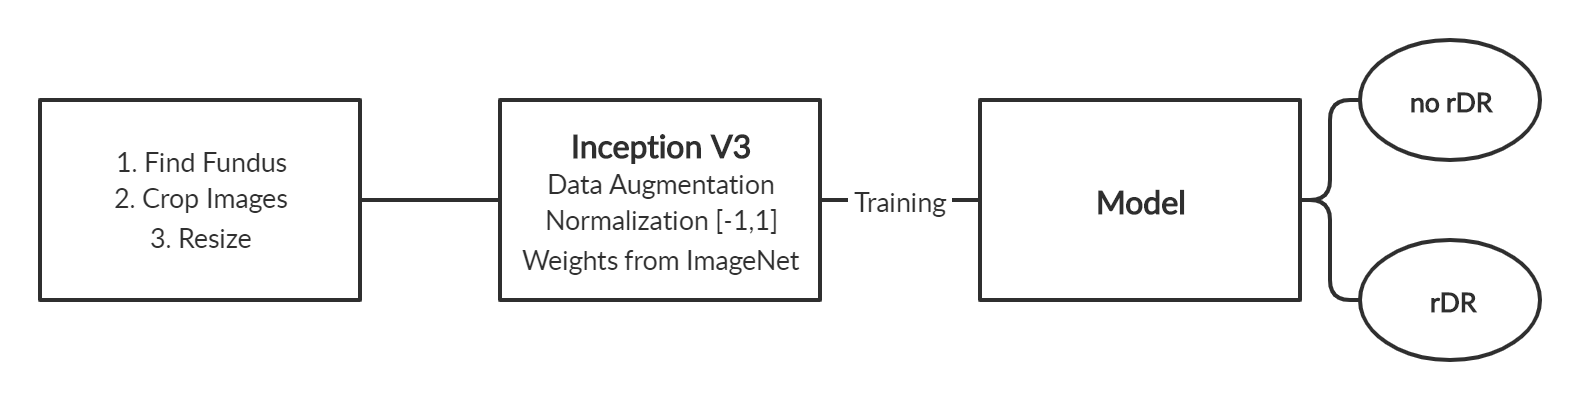
\includegraphics[width=1\linewidth]{cnn_flow.png} \caption{Συνοπτική περιγραφή του πειράματος CNN με εικόνες RGB}
\label{figure:cnnflow}  
\end{figure}



\subsection{Αύξηση Δεδομένων και Επεξεργασία Εικόνων}
\label{subsec:5.1.2}

Επίσης, έγινε αύξηση δεδομένων ώστε να επιτευχθεί καλύτερη ακρίβεια και μείωση της υπερεκπαιδευσης. Σε κάθε εποχή οι εικόνες μετασχηματίζονται με τυχαίο τρόπο ωστόσο ο  αριθμός των εικόνων παραμένει ίδιος. Άρα πρέπει να γίνει σαφές ότι οι εικόνες δεν αυξάνονται αλλά σε κάθε εποχή κάθε εικόνα υφίσταται ένα σύνολο μετασχηματισμών. Αύξηση δεδομένων αποτελείται μόνο στο σύνολο εκπαίδευσης και όχι στα σύνολο επικύρωσης και ελέγχου.

\subsubsection{Περιστροφή}
\label{subsubsec:5.1.2.1}


Επιλέχθηκε η χρήση αύξησης δεδομένων με περιστροφή ως προς το κέντρο της εικόνας κατά τυχαία γωνία στο διάστημα [0$^\circ$,360$^\circ$]. Σε πρώτη θεώρηση οι περιεστρεμμένες εικόνες φαίνονται μη ρεαλιστικές, καθώς η τυπική δομή περιέχει οπτικό δίσκο και ωχρά κηλίδα σε κάποιες σχετικά αναμενόμενες θέσεις  μέσα στην εικόνα. Για παράδειγμα μία ωχρά κηλίδα στο πάνω μέρος του αμφιβληστροειδούς θα ήταν μη ρεαλιστική. Ωστόσο, όπως αποδείχθηκε και με πειράματα με χρήση περιστροφής των εικόνων  δίνονται πολύ καλύτερα αποτελέσματα καθώς η ασθένεια είναι σταθερή σε σχέση με τη περιστροφή. Τέλος να σημειωθεί, ότι η αύξηση δεδομένων με περιστροφή έχει διττό ρόλο καθώς μειώνει το υπερεκπαίδευση και αυξάνει την ακρίβεια.



\subsubsection{Προσαρμογή Κορεσμού και Απόχρωσης}
\label{subsubsec:5.1.2.2}

Για την προσαρμογή του κορεσμού και της απόχρωσης μεταφέραμε την RGB εικόνα στο HSV χρωματικό χώρο\cite{HSV}. Ο χρωματικός χώρος HSV(απόχρωση, κορεσμός, φωτεινότητα) αποτελεί εναλλακτική αναπαράσταση του χρωματικού χώρου RGB και σχεδιάστηκε για να αναπαραστήσει καλύτερα  τον τρόπο με τον  οποίο οι άνθρωποι αντιλαμβάνονται το χρώμα. Η αναπαράσταση του HSV χρωματικού χώρου έχει κυλινδρική γεωμετρία όπως φαίνεται στην εικόνα \ref{figure:hsv}. Στον HSV χρωματικό χώρο τα χρώματα περιγράφονται μέσω του καναλιού της απόχρωσης(Hue). Η ποσότητα του γκρι σε ένα  χρώμα περιγράφεται μέσω του καναλιού του κορεσμού(Saturation) και η ένταση του χρώματος αναπαρίσταται με το κανάλι φωτεινότητας(Value).



\begin{figure}[!h]
    \centering
      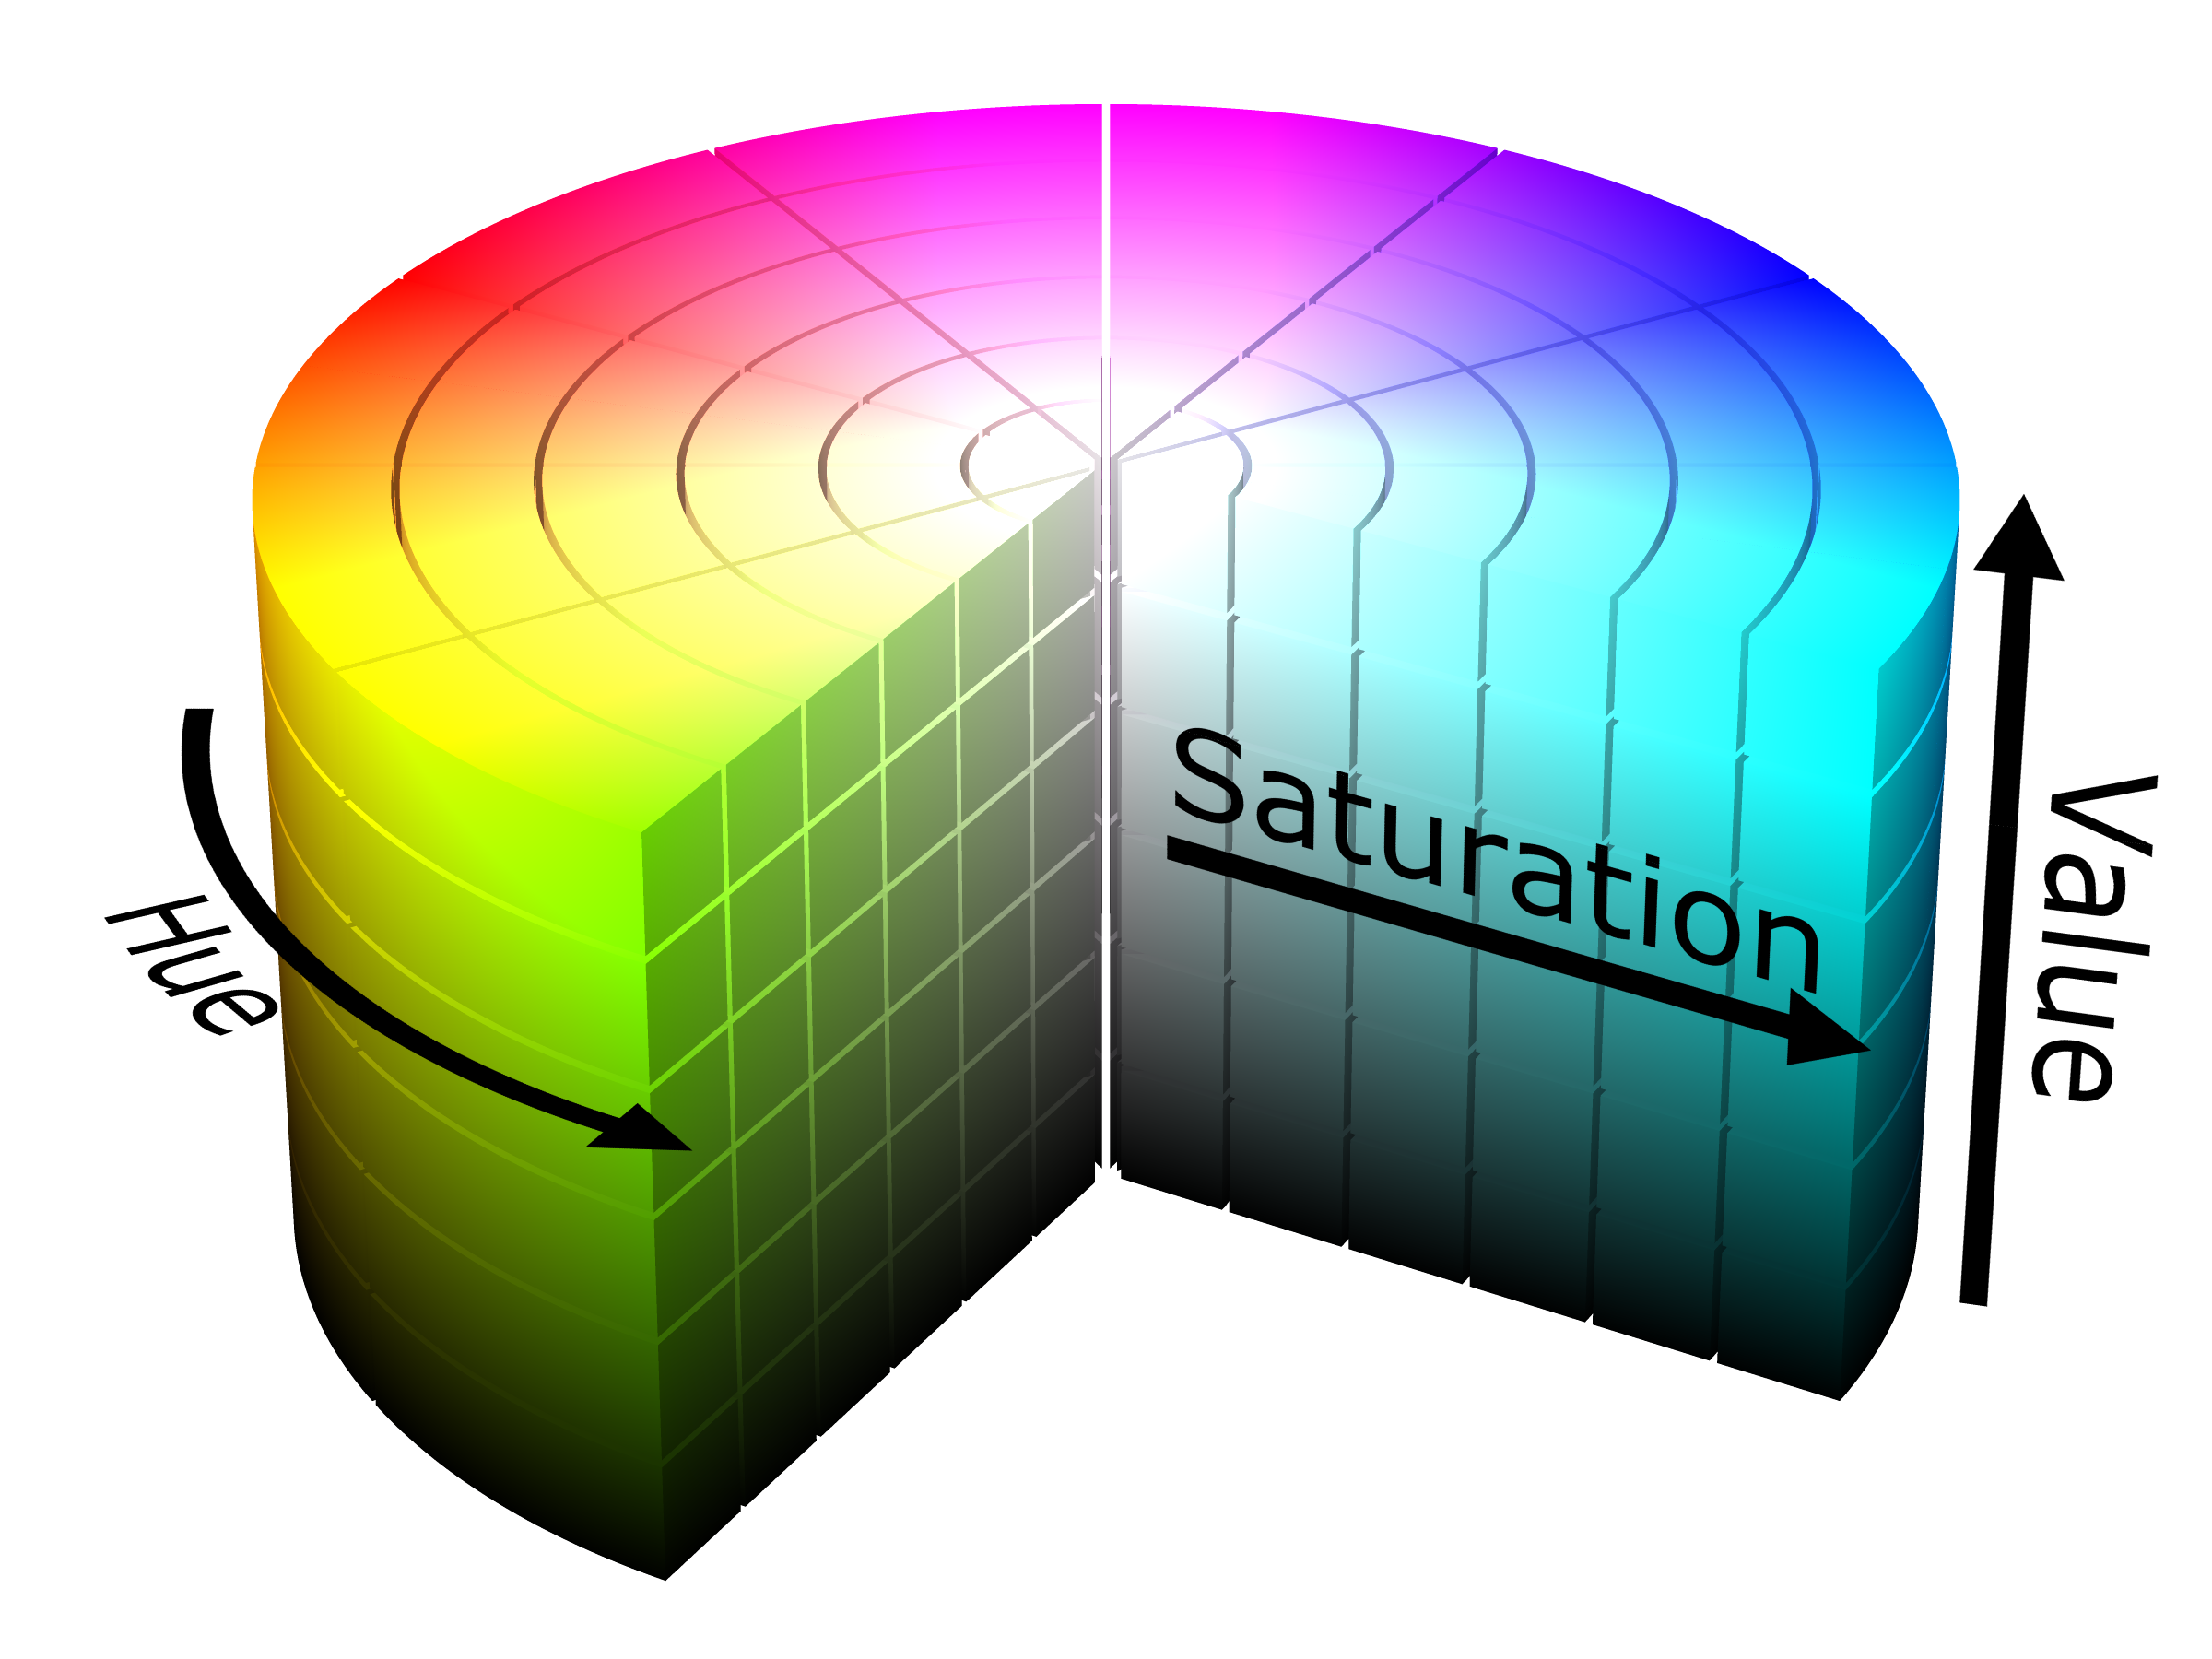
\includegraphics[width=0.6\linewidth]{hsv.png} \caption{Χρωματικός χώρος HSV}
      \label{figure:hsv}    
  \end{figure}


Το κανάλι της απόχρωσης αποτελεί τη γωνιακή συντεταγμένη. Ξεκινώντας από το κόκκινο στις 0$^\circ$ περνάει από το κίτρινο, το πράσινο, το γαλάζιο, το μπλε και το μωβ και καταλήγει μετά από πλήρη περιστροφή στο κόκκινο ξανά. Το κανάλι κορεσμού αποτελεί την ακτινική διάσταση και περιγράφει την ποσότητα γκρι σε ένα συγκεκριμένο χρώμα. Όσο πιο κοντά στο 0, τόσο πιο μεγάλη ποσότητα γκρι περιέχεται στο χρώμα. Το κανάλι φωτεινότητας  αποτελεί τη διάσταση του ύψους και περιγράφει την ένταση του χρώματος στο κλίμακα [0-100], όπου το 0 αντιστοιχίζεται στο μαύρο ενώ στο 100 έχουμε την μεγαλύτερη ένταση του χρώματος. Παρακάτω θα περιγραφεί ο τρόπος προσαρμογής της απόχρωσης και του κορεσμού. Τα διαστήματα τιμών για το κάθε κανάλι καθορίζονται από τον τρόπο αναπαράστασης του HSV χρωματικού χώρου στη Python.

Για την προσαρμογή της απόχρωσης προστίθεται σε όλα τα εικονοστοιχεία της εικόνας ένας σταθερός όρος στο διάστημα [0-5]. Η απόχρωση παίρνει τιμές στο διάστημα [0,179] και η αναπαράσταση της είναι κυκλική. Για τα εικονοστοιχεια των οποίων η τιμή της απόχρωσης είναι μεγαλύτερη από 180, επιστρέφεται το υπόλοιπο της διαίρεσης με το 180.

Για την προσαρμογή του κορεσμού προστίθεται σε όλα τα εικονοστοιχεία της εικόνας ένας σταθερός όρος στο διάστημα [-25, 25]. Το κανάλι κορεσμού παίρνει τιμές στο διάστημα [0, 255] οπότε  οι αρνητικές τιμές εικονοστοιχείων ή οι τιμές που ξεπερνούν το 255, τίθενται στο 0 και 255 αντίστοιχα. Να σημειωθεί ότι το διάστημα των σταθερών όρων  για τη προσαρμογή και την αντίθεση βρέθηκε πειραματικά ώστε να παράγονται ρεαλιστικά αποτελέσματα, δηλαδή εικόνες που θα μπορούσαν να ανήκουν στο σύνολο δεδομένων. 

\subsubsection{Προσαρμογή Φωτεινότητας και Αντίθεσης}
\label{subsubsec:5.1.2.3}


Για την προσαρμογή της φωτεινότητας και της αντίθεσης χρησιμοποιήθηκε ο μετασχηματισμός $α \cdot  f(i, j) +β$ που σύμφωνα με την βιβλιογραφία αλλάζει ταυτόχρονα φωτεινότητα και αντίθεση. \cite{Szeliski} \cite{Changing}. Η συνάρτηση $f(i,j)$ αναπαριστά την τιμή του μετασχηματισμένου εικονοστοιχείου (i,j) και τα α και β αποτελούν τις παραμέτρους προσαρμογής αντιθεσης και φωτεινοτητας, αντίστοιχα. 

Η χρήση του παραπάνω  μετασχηματισμού μπορεί να γίνει πιο κατανοητή με τα παρακάτω ιστογράμματα. Στον οριζόντιο άξονα ενός ιστογράμματος τοποθετούνται τα επίπεδα χρώματος μιας εικόνας, πχ για 8 bit εικόνα υπάρχουν 256 επίπεδα. Στον κατακόρυφο άξονα τοποθετείται ο αριθμός των εικονοστοιχείων που βρίσκεται σε ένα συγκεκριμένο επίπεδο χρώματος. Αν προστεθεί μια σταθερή θετική τιμή β σε όλα τα εικονοστοιχεία μίας εικόνας, τότε τα εικονοστοιχεία με τιμές μεγαλύτερες του 255 θα αντιστοιχιστούν στο 255. Αν προστεθεί μια σταθερή αρνητική τιμή β τότε τα εικονοστοιχεία με τιμές μικρότερες του 0 θα αντιστοιχιστούν στο 0. Με αυτόν τον τρόπο, στην πρώτη περίπτωση θα αυξηθεί η φωτεινότητα καθώς πιο πολλά εικονοστοιχεια θα βρεθούν στο 255, ενώ στη δεύτερη περίπτωση θα μειωθεί η φωτεινότητα καθώς πιο πολλά εικονοστοιχεια θα βρεθούν στο 0. Η αναπαράσταση της πρώτης περίπτωσης παρουσιάζεται στην εικόνα \ref{figure:b}. Με γκρι είναι το αρχικό ιστόγραμμα της εικόνας και με μαύρο το καινούριο ιστόγραμμα μετά από προσθήκη σταθερής θετικής τιμής σε όλα τα εικονοστοιχεια της εικόνας.

\begin{figure}[!h]
    \centering
      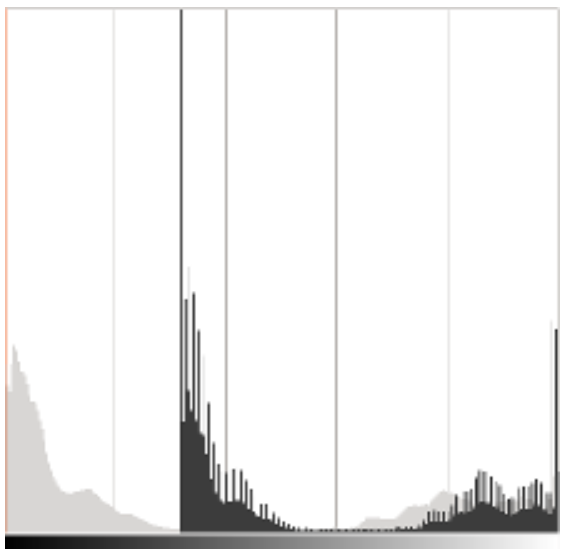
\includegraphics[width=0.4\linewidth]{b.PNG} \caption{Ιστόγραμμα εικόνας πριν(γκρι) και μετά(μαύρο) την πρόσθεση σταθερής τιμής b>0}
      \label{figure:b}    
  \end{figure}
  
Όσον αφορά την παράμετρο α, αυτή ρυθμίζει την έκταση  των τιμών στον οριζόντιο άξονα του ιστογράμματος. Για τιμές α<1, οι τιμές του οριζόντιου άξονα συμπιέζονται και η αντίθεση της εικόνας μειώνεται, καθώς περισσότερα εικονοστοιχεια αντιστοιχίζονται σε ίδιες τιμές του οριζόντιου άξονα. Αντίθετα για τιμές α>1 το ιστόγραμμα απλώνει και η εικόνα παρουσιάζει μεγαλύτερη αντίθεση. Η αναπαράσταση της παραπάνω περιγραφής παρουσιάζεται στην εικόνα \ref{figure:a}. Με γκρι είναι το αρχικό ιστόγραμμα της εικόνας ενώ με μαύρο το καινούριο ιστόγραμμα μετά από τον πολλαπλασιασμό με σταθερή θετική τιμή α<1 σε όλα τα εικονοστοιχεια της εικόνας.

\begin{figure}[!h]
    \centering
      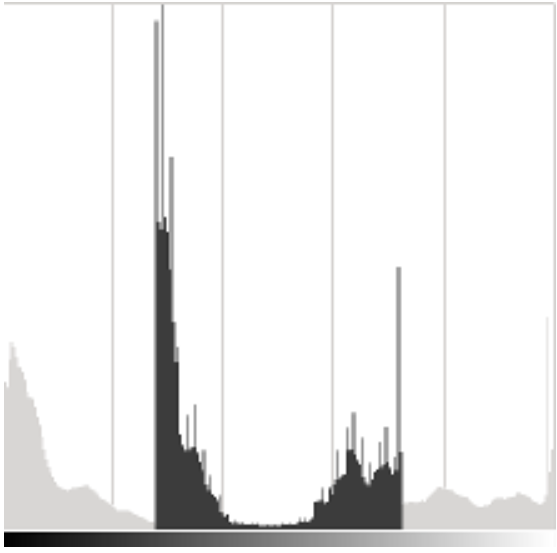
\includegraphics[width=0.4\linewidth]{a.PNG} \caption{Ιστόγραμμα εικόνας πριν(γκρι) και μετά(μαύρο) τον πολλαπλασιασμό με σταθερή τιμή α<1}
      \label{figure:a}    
  \end{figure}


Για την παρούσα διπλωματική, το εύρος τιμών για την παράμετρο προσαρμογής  αντίθεσης ορίστηκε στο διάστημα [0.5, 1.5] και για την παράμετρο προσαρμογής φωτεινότητας στο διάστημα [-40,40]. Μετά τον μετασχηματισμό, οι  αρνητικές τιμές εικονοστοιχείων ή οι τιμές που ξεπερνούν τα 255, τέθηκαν 0 και 255, αντίστοιχα. Στη περίπτωση προσαρμογής φωτεινότητας και αντίθεσης το διάστημα των παραμέτρων προσαρμογής βρέθηκε πειραματικά με γνώμονα την παραγωγή ρεαλιστικών εικόνων, δηλαδή εικόνων που θα μπορούσαν να ανήκουν στο σύνολο δεδομένων. 

\subsubsection{Κανονικοποίηση εικόνων}
\label{subsubsec:5.1.2.4}

Λόγω της αρχικοποίησης με έτοιμα βάρη, οι εικόνες εισόδου πρέπει να κανονικοποιηθούν στο [-1, 1]. Στην \ref{eq:norm}  δίνεται η διαδικασία που ακολουθείται για την τελική κανονικοποίηση στο [-1, 1].  Τα εικονοστοιχεία των αρχικών εικόνων  παίρνουν τιμές στο διάστημα [0, 255]. Αρχικά κάθε εικονοστοιχείο της εικόνας διαιρείται με 255 έτσι ώστε η εικόνα να κανονικοποιηθεί στο [0,1]. Στη συνέχεια αφαιρείται από κάθε εικονοστοιχείο η τιμή 0.5, και η εικόνα παίρνει τιμές στο [-0.5, 0.5]. Τέλος τα εικονοστοιχεια πολλαπλασιάζονται με την τιμή 2, άρα η εικόνα καταλήγει στην επιθυμητή κανονικοποίηση στο [-1, 1].


\begin{equation}
\label{eq:norm}
\begin{split}
x /= 255\\
x -= 0.5\\
x *= 2
\end{split}
\end{equation}

όπου x η εικόνα εισόδου. Όλες οι παραπάνω πράξεις εφαρμόζονται σε κάθε εικονοστοιχείο της εικόνας.



\subsubsection{Συνάρτηση επεξεργασίας}
\label{subsubsec:5.1.2.5}

Το Keras, εκτός των έτοιμων συναρτήσεων για μετασχηματισμό των δεδομένων κατά τη διάρκεια της εκπαίδευσης,  επιτρέπει τη χρήση μιας συνάρτησης επεξεργασίας που θα καλείται για κάθε εικόνα κάθε εποχή και μπορεί να περιέχει οποιοδήποτε κώδικα. 
Η συνάρτηση επεξεργασίας είναι ένα από τα πιο σημαντικά χαρακτηριστικά που προσφέρει το Keras για αύξηση δεδομένων και συγχρόνως δίνει τη δυνατότητα πειραματισμό με διαφόρους μετασχηματισμούς (αλλαγή χρωματικού χώρου, εξισορρόπηση χρώματος) χωρίς να απαιτείται ο μετασχηματισμός των εικόνων και η αποθήκευση τους πριν την έναρξη της εκπαίδευσης. 
Στην συνάρτηση μετασχηματισμού αρχικά εφαρμόζεται η περιστροφή της εικόνας, η οποία εξηγήθηκε παραπάνω, στις μισές εικόνες σε κάθε εποχή με τυχαία επιλογή των εικόνων. Έπειτα εφαρμόζονται προσαρμογή Κορεσμού-Απόχρωσης και Φωτεινότητας-Αντίθεσης και σε αυτή την περίπτωση οι μετασχηματισμοί εφαρμόζονται στις μούσες εικόνες σε κάθε εποχή με τυχαία επιλογή των εικόνων επιπλέον οι μετασχηματισμοί Κορεσμού-Απόχρωσης και Φωτεινότητας-Αντίθεσης γίνονται με τυχαία σειρά. Στην εικόνα\ref{figure:viz2}  παρουσιάζονται κάποιες εικόνες που έχουν υποστεί τους παραπάνω μετασχηματισμούς. Τέλος, εφαρμόζεται η συνάρτηση κανονικοποίησης στο διάστημα [-1,1]. 

\begin{figure}[!h]
    \centering
      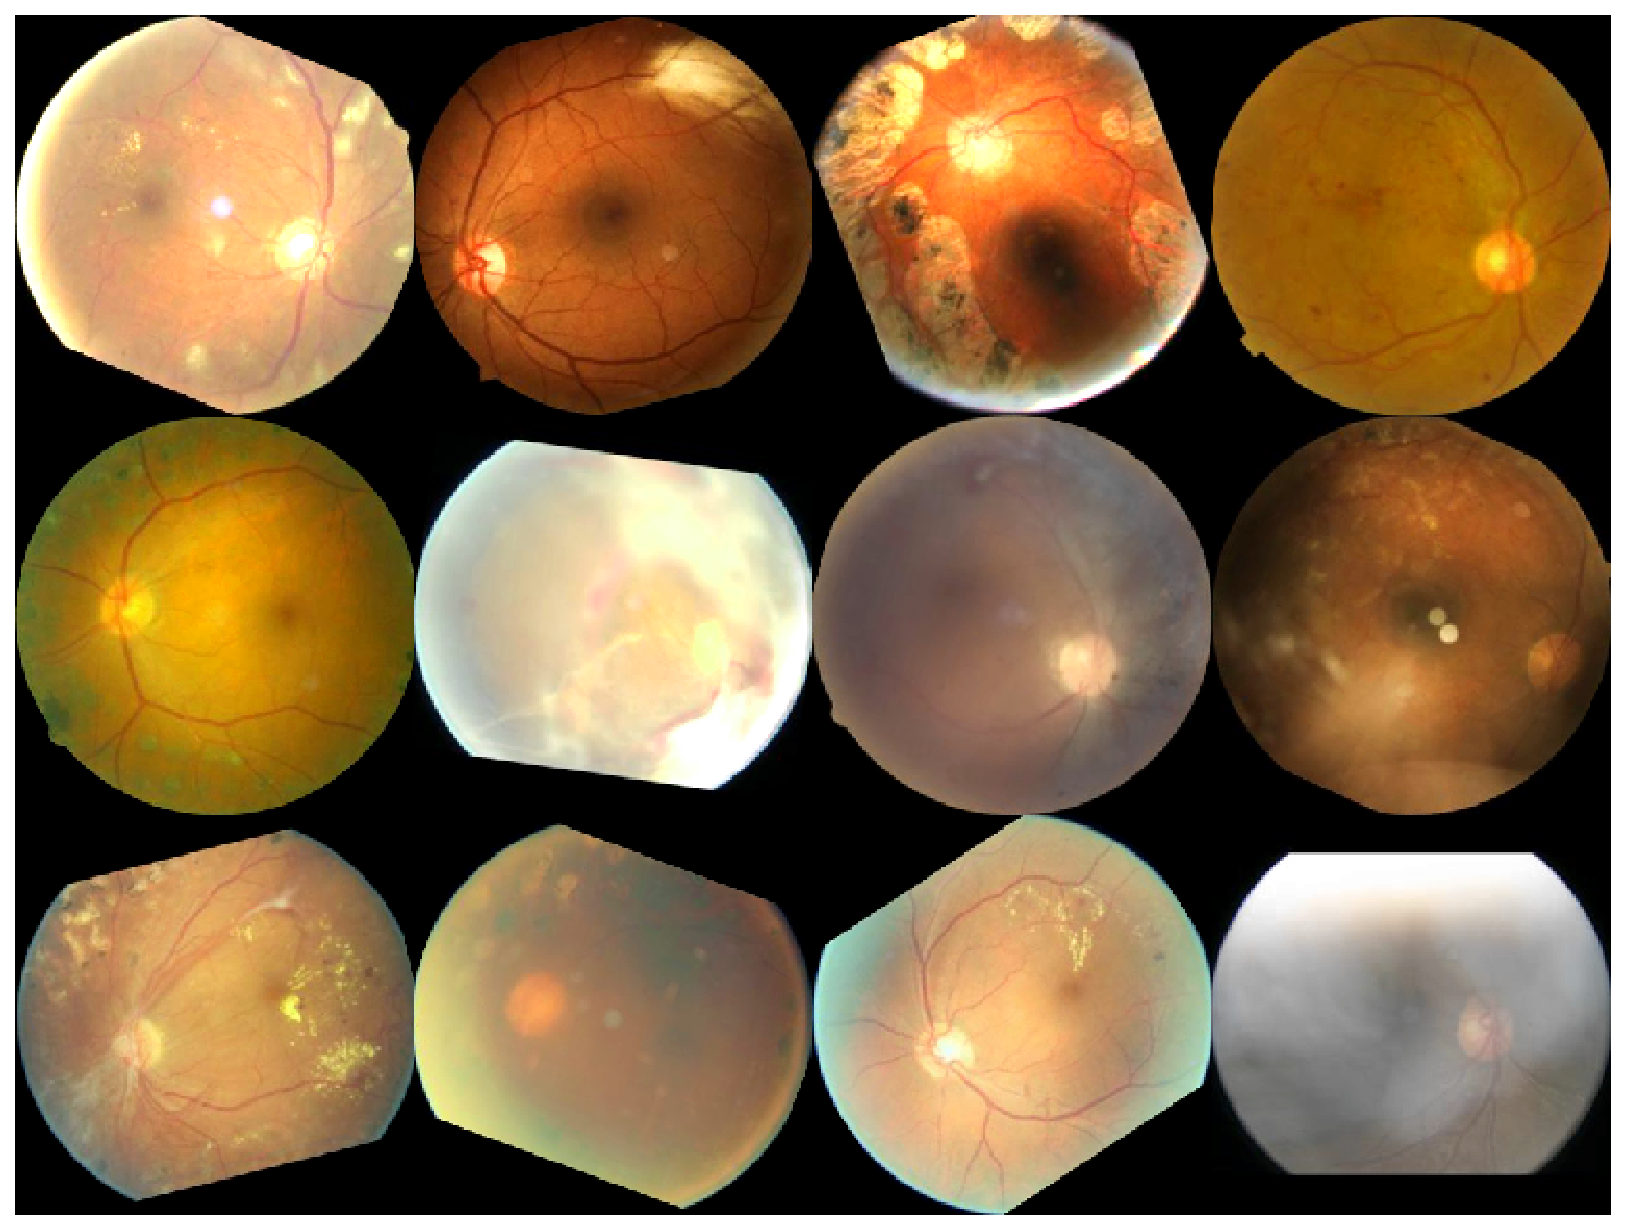
\includegraphics[width=1\linewidth]{vis2.pdf} \caption{Εικόνες που έχουν υποστεί περιστροφή και προσαρμογή φωτεινότητας, αντίθεσης, απόχρωσης και κορεσμού}
\label{figure:viz2}  
\end{figure}




\section{CNN με ταξινομητή SVM}
\label{sec:5.2}


Στο πείραμα με ταξινομητή Support Vector Machine ακολουθήθηκε η εξής διαδικασία. Μετά την εκπαίδευση  του νευρωνικού όπως εξηγήθηκε στην παραπάνω παράγραφο, δόθηκαν ως είσοδος στο μοντέλο τα σύνολα εκπαίδευσης και επικύρωσης και ανακτήθηκε ο χάρτης χαρακτηριστικών από το πρώτο πλήρη συνδεδεμένο επίπεδο με 2048 νευρώνες για κάθε εικόνα. Ο παραπάνω χάρτης χαρακτηριστικών είναι ένα διάνυσμα με 2048 νευρώνες και περιέχει την πληροφορία για τα χαρακτηριστικά που εντοπίστηκαν στην κάθε εικόνα. Έπειτα, το διάνυσμα με τις αντίστοιχες κλάσεις δόθηκε ως είσοδο στο μοντέλο SVM.
  Ουσιαστικά, αντί να δοθούν οι εικόνες στο ταξινομητή SVM, το οποίο μάλιστα θα ήταν αδύνατο λόγω του μεγάλου μεγέθους τους αλλά και της χωρικής πληροφορίας που περιέχουν και η οποία θα χάνονταν, δίνονται οι χάρτες χαρακτηριστικών με την αντίστοιχη κλάση που άνηκε η κάθε εικόνα από την οποία εξάχθηκαν. Επιπλέον, η πληροφορία των χαρτών χαρακτηριστικών είναι εξειδικευμένη στην ύπαρξη ή όχι rDR, καθώς τον νευρωνικό εκπαιδεύτηκε βάση αυτών των κλάσεων. Για την ταξινόμηση χρησιμοποιήθηκε ένας γραμμικός ταξινομητής SVM και ένας ταξινομητής με μη γραμμική συνάρτηση πυρήνα Radial basis. Στην εικόνα \ref{figure:cnnflowsvm} δίνεται μία συνοπτική περιγραφή του πειράματος CNN με ταξινομητή SVM.
  

  
\begin{figure}[!h]
    \centering
      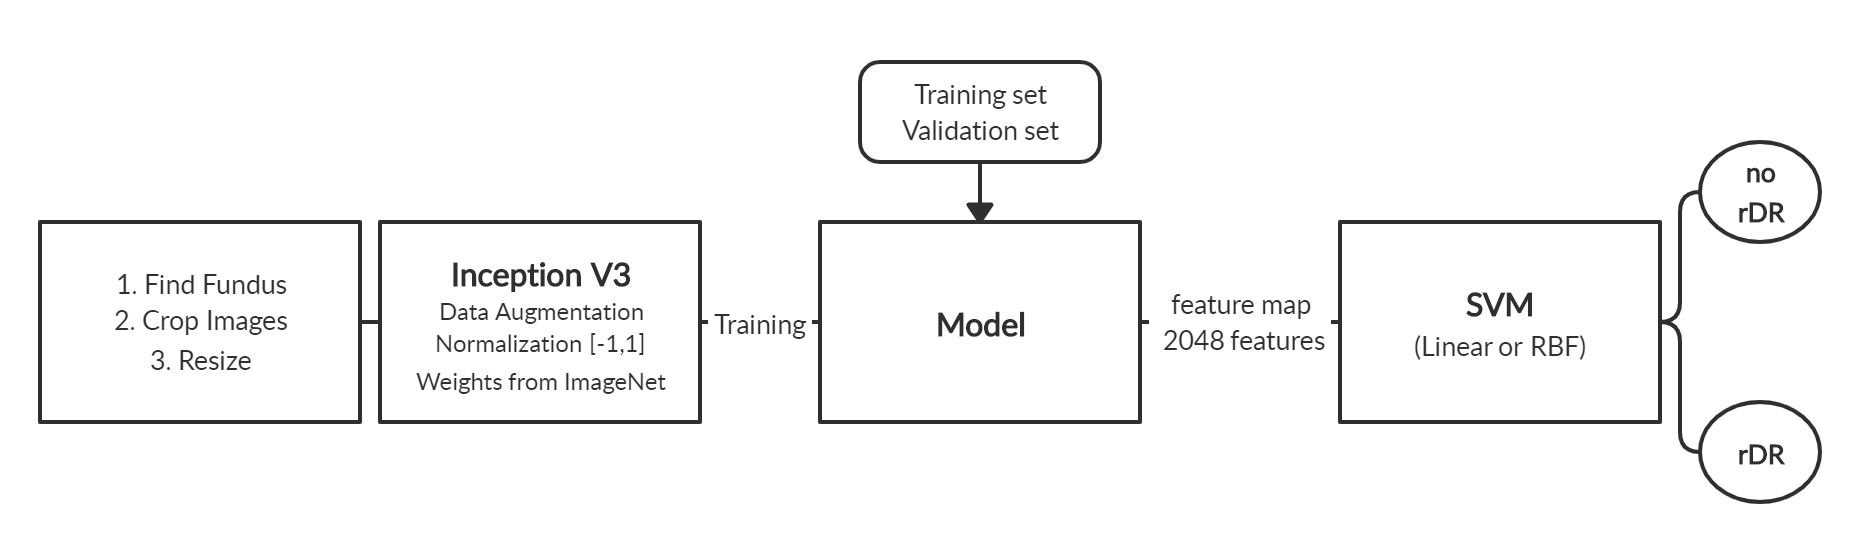
\includegraphics[width=1\linewidth]{cnn_svm_flow.png} \caption{Συνοπτική περιγραφή του πειράματος CNN με ταξινομητή SVM}
\label{figure:cnnflowsvm}  
\end{figure}


\section{Ensemble}
\label{sec:5.3}

Τα μοντέλα Ensemble συνδυάζουν τις αποφάσεις από πολλά μοντέλα για να βελτιώσουν την συνολική απόδοση. Επιπλέον βοηθούν στη βελτίωση της σταθερότητας και της ακρίβειας. Στην παρούσα διπλωματική εξετάστηκαν δύο μέθοδοι ensemble, το ensemble μέσης τιμής και ensemble με ψηφοφορία.
Για τις παραπάνω μεθόδους χρησιμοποιήθηκαν 9 μοντέλα. Τα 9 μοντέλο εκπαιδεύτηκαν για 40 εποχές, με μέγεθος πακέτου(batch size) 8 ή 32 εικόνες και διάφορους ρυθμούς εκμάθησης. Κάθε εποχή πήρε περίπου 11 λεπτά και η διάρκεια εκπαίδευσης ήταν περίπου 7,5 ώρες/μοντέλο. Να σημειωθεί ότι λόγω της αύξησης δεδομένων και των τυχαίων εικόνων που παράγονται κάθε φορά, μοντέλα που έτρεξαν με ίδιο μέγεθος πακέτου και ρυθμό εκμάθησης είναι δυνατόν να  παρουσιάσουν μικρές διαφορές ως προς το τελικο αποτέλεσμα. Αυτό είναι λογικό καθώς σε ένα πείραμα μπορεί να παραχθούν  εικόνες που θα κατευθύνουν καλύτερα το νευρωνικό στο να ανακαλύψει τα χαρακτηριστικά σχετικά με την ύπαρξη ή όχι της rDR.   
 
\subsection{Ensemble Μέσης Τιμής}
\label{subsec:5.3.1}
Στο ensemble μέσης τιμής αρχικά υπολογίζονται οι προβλέψεις (πιθανότητες) κάθε μοντέλου για το σύνολο ελέγχου. Έπειτα, για κάθε εικόνα αθροίζονται οι προβλέψεις από κάθε μοντέλο και διαιρούνται με τον αριθμό των μοντέλων. Η διαδικασία αυτή ακολουθείται για όλες τις εικόνες του συνόλου ελέγχου. Στο τέλος αυτής της διαδικασίας θα έχουν υπολογιστεί οι προβλέψεις του μοντέλου ensemble μέσης τιμής για το σύνολο ελέγχου. Όπως και στα απλά μοντέλα, για διάφορα κατώφλια υπολογίζεται η μετρική AUC και εξάγονται τα σημεία υψηλής ευαισθησίας και εξειδίκευσης, όπως επίσης και το βέλτιστο σημείο.  Στην εικόνα \ref{figure:avg} παρουσιάζεται η δομή του Ensemble μέσης τιμής.


\begin{figure}[!h]
    \centering
      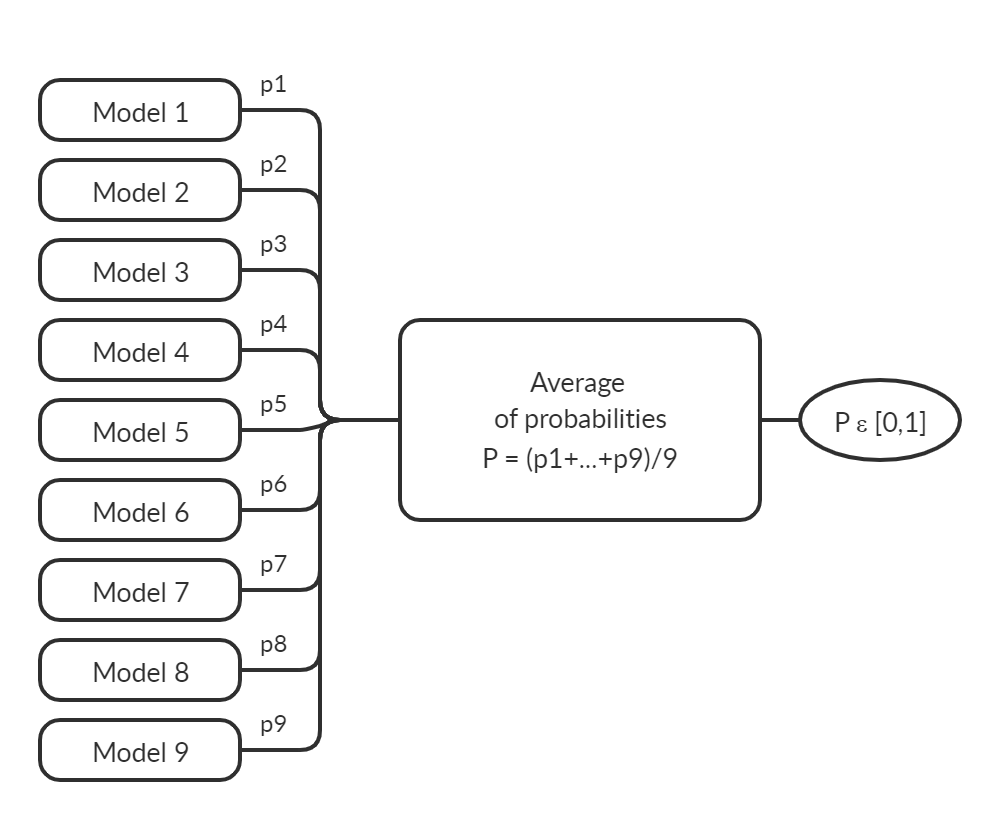
\includegraphics[width=0.6\linewidth]{avg.png} \caption{Ensemble μέσης τιμής για 9 μοντέλα}
      \label{figure:avg}    
  \end{figure}
 
\subsection{Ensemble με Ψηφοφορία}
\label{subsec:5.3.2}
Στο ensemble με ψηφοφορία αρχικά υπολογίζονται οι προβλέψεις κάθε μοντέλου για το σύνολο ελέγχου. 
Έπειτα για κάθε μοντέλο ακολουθείται η εξής διαδικασία: για διάφορα κατώφλια υπολογίζεται για κάθε εικόνα, η κλάση στην οποία ανήκει. Αφού υπολογιστούν τα παραπάνω. Για να υπολογιστεί η κλάση στην οποία ανήκει κάθε εικόνα για ένα συγκεκριμένα κατώφλι, το 9 μοντέλα ψηφίζουν. Αν για μία εικόνα πάνω από τα 4 μοντέλα έχουν ψηφίσει μια συγκεκριμένη κλάση, τότε αυτή είναι η νέα κλάση της εικόνας. Η παραπάνω διαδικασία θα επαναληφθεί για όλα τα κατώφλια. Στον τέλος βάση των κατωφλιών και των νέων κλάσεων των εικόνων, προκύπτει η μετρική AUC και τα σημεία υψηλής ευαισθησίας και εξειδίκευσης, όπως επίσης και το βέλτιστο σημείο. Στην εικόνα \ref{figure:voting} παρουσιάζεται η δομή του Ensemble με ψηφοφορία.

\begin{figure}[!h]
    \centering
      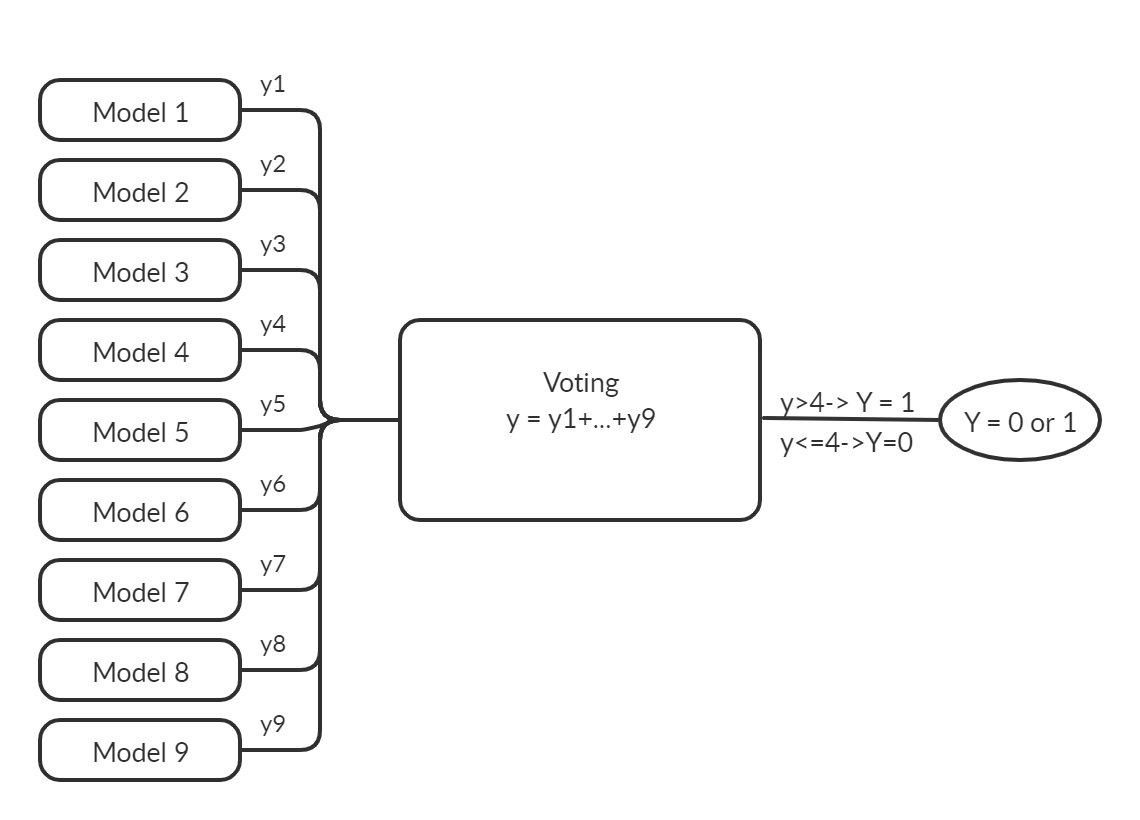
\includegraphics[width=0.6\linewidth]{voting.png} \caption{Ensemble με ψηφοφορία για 9 μοντέλα για συγκεκριμένο κατώφλι t}
      \label{figure:voting}    
\end{figure}
  
  



\section{Επιπλέον Πειράματα}
\label{sec:5.4}
Σε αυτή την παράγραφο θα γίνει αναφορά σε ορισμένα πειράματα  που πραγματοποιήθηκαν με σκοπό τη βελτίωση των αποτελεσμάτων, ωστόσο έδωσαν παρόμοια ή κατώτερα αποτελέσματα. Κρίνεται σκόπιμο να γίνει αναφορά σε αυτά τα πειράματα, ώστε να υπάρχει η γνώση της μη αποτελεσματικότητα τους.


\subsection{Αλλαγή από RGB σε άλλους Xρωματικούς Xώρους}
\label{subsec:5.4.1}
Δοκιμάστηκε ο μετασχηματισμός των εικόνων από RGB στους χρωματικούς χώρους YUV και Lab. Ο χρωματικός χώρος YUV προέρχεται από γραμμικό μετασχηματισμό των RGB  καναλιών όποτε πιθανότατα η μετατροπή αυτή δεν προσφέρει κάποια καινούργια πληροφορία στο νευρωνικό. Αντίθετα, ο χρωματικός χώρος Lab δεν προέρχεται από γραμμικό μετασχηματισμό των RGB καναλιών και ίσως θα μπορούσε να αποδώσει καλύτερα την πληροφορία των εικόνων.  Όπως αποδείχθηκε  πειραματικά η μετατροπή των εικόνων στους παραπάνω χρωματικούς χώρους έδωσε παρόμοια, με τον χρωματικό χώρο RGB, αποτελέσματα.

\subsection{Μετασχηματισμός Clahe}
\label{subsec:5.4.2}
Για την ενίσχυση της τοπικής αντίθεσης των εικόνων δοκιμάστηκε ο μετασχηματισμός Contrast Limited Adaptive histogram equalization(Clahe), μία παραλλαγή του μετασχηματισμού Adaptive histogram equalization, με μέγεθος γειτονιάς 8x8\cite{clahe}. Ο μετασχηματισμός εφαρμόστηκε με τις εξής μορφές: 1. Εφαρμογή μετασχηματισμού  σε κάθε ένα από τα RGB κανάλια ξεχωριστά, 2.  Μετασχηματισμός των εικόνων σε YUV χρωματικό χώρο, εφαρμογή Clahe στο κανάλι Y και επιστροφή στο RGB χρωματικό χώρο  3.  Μετασχηματισμός των εικόνων σε Lab χρωματικό χώρο, εφαρμογή Clahe στο κανάλι L και επιστροφή στο RGB χρωματικό χώρο. 

Επιπλέον, δοκιμάστηκε αντί των 3 καναλιών RGB χρήση 3 καναλιών με το πρώτο κανάλι να περιέχει το μετασχηματισμό Clahe της ασπρόμαυρης εικόνας, το δεύτερο εικόνες εντροπίας και το τρίτο το Y κανάλι από το μετασχηματισμό YUV. Οι εικόνες εντροπίας υπολογίζονται αφού πρώτα μετατραπεί η εικόνα σε κλίμακα του γκρι (grayscale) και στη συνέχεια αντικατασταθεί κάθε εικονοστοιχείο με την τιμή της εντροπίας σε μία γειτονιά του εικονοστοιχείου.

\subsection{Αύξηση Δεδομένων πριν την Είσοδο στο Νευρωνικό}
\label{subsec:5.4.3}
Δοκιμάστηκε και η αύξηση δεδομένων πριν δοθούν στο νευρωνικό ώστε να υπάρχει ίδιος αριθμός εικόνων σε κάθε κλάση. Έτσι στην κλάση rDR που υπάρχουν πολύ λιγότερες εικόνες παράχθηκαν νέες εικόνες  από τις ήδη υπάρχουσες. Οι νέες εικόνες παράχθηκαν με αλλαγή της φωτεινότητας, του κορεσμού, της απόχρωσης και της αντίθεσης των εικόνων της κλάσης rDR. Από αυτή τη διαδικασία o  χρόνος εκπαίδευσης αυξήθηκε αρκετά χωρίς ωστόσο να βελτιωθούν τα αποτελέσματα. Να σημειωθεί ότι και σε αυτό το πείραμα έγινε αύξηση δεδομένων κατά τη διάρκεια της εκπαίδευσης.

\subsection{Χρήση Ασπρόμαυρης Μάσκας}
\label{subsec:5.4.4}
Δοκιμάστηκε η χρήση δύο ασπρόμαυρων μασκών για τις δύο μορφές εικόνων. Η μία μάσκα περιείχε ολόκληρο τον αμφιβληστροειδή ενώ η δεύτερη είχε κομμένο το πάνω και κάτω μέρος κατά αναλογία με τις εικόνες του συνόλου δεδομένων Kaggle. Στην εικόνα \ref{figure:bl} παρουσιάζονται οι δύο μάσκες. 


\begin{figure}[!h]
\centering
\begin{subfigure}{.5\textwidth}
  \centering
  
\includegraphics[scale=0.5]{bl.png}
  \caption{Μάσκα 1}
  \label{fig:bl1}
\end{subfigure}
\qquad
\begin{subfigure}{.5\textwidth}
  \centering
  
\includegraphics[scale=0.5]{bl2.png}
  \caption{Μάσκα 2}
  \label{fig:bl2}
\end{subfigure}
\caption{Μάσκες}
\label{figure:bl}
\end{figure}

Κάθε εικόνα πολλαπλασιάστηκε με την αντίστοιχη μάσκα και το αποτέλεσμα έδωσε μία πιο σταθερή δομή στις εικόνες και ένα ομοιόμορφο μαύρο φόντο για τις εικόνες που είχαν εικονοστοιχία διάφορα του [0,0,0] στο φόντο. Με την εφαρμογή των παραπάνω μασκών χάνεται ένα κομμάτι της πληροφορίας της εικόνας το οποίο όμως δεν θεωρείται σημαντικό καθώς  η ασθένεια δεν εντοπίζεται συνήθως στα άκρα του αμφιβληστροειδούς. Κάποια ενδεικτικά δείγματα των εικόνων που παρήχθησαν παρουσιάζονται στην \ref{figure:stable}. Η εφαρμογή των μασκών στις εικόνες δεν έδωσε καλύτερα αποτελέσματα.

\begin{figure}[!h]
    \centering
      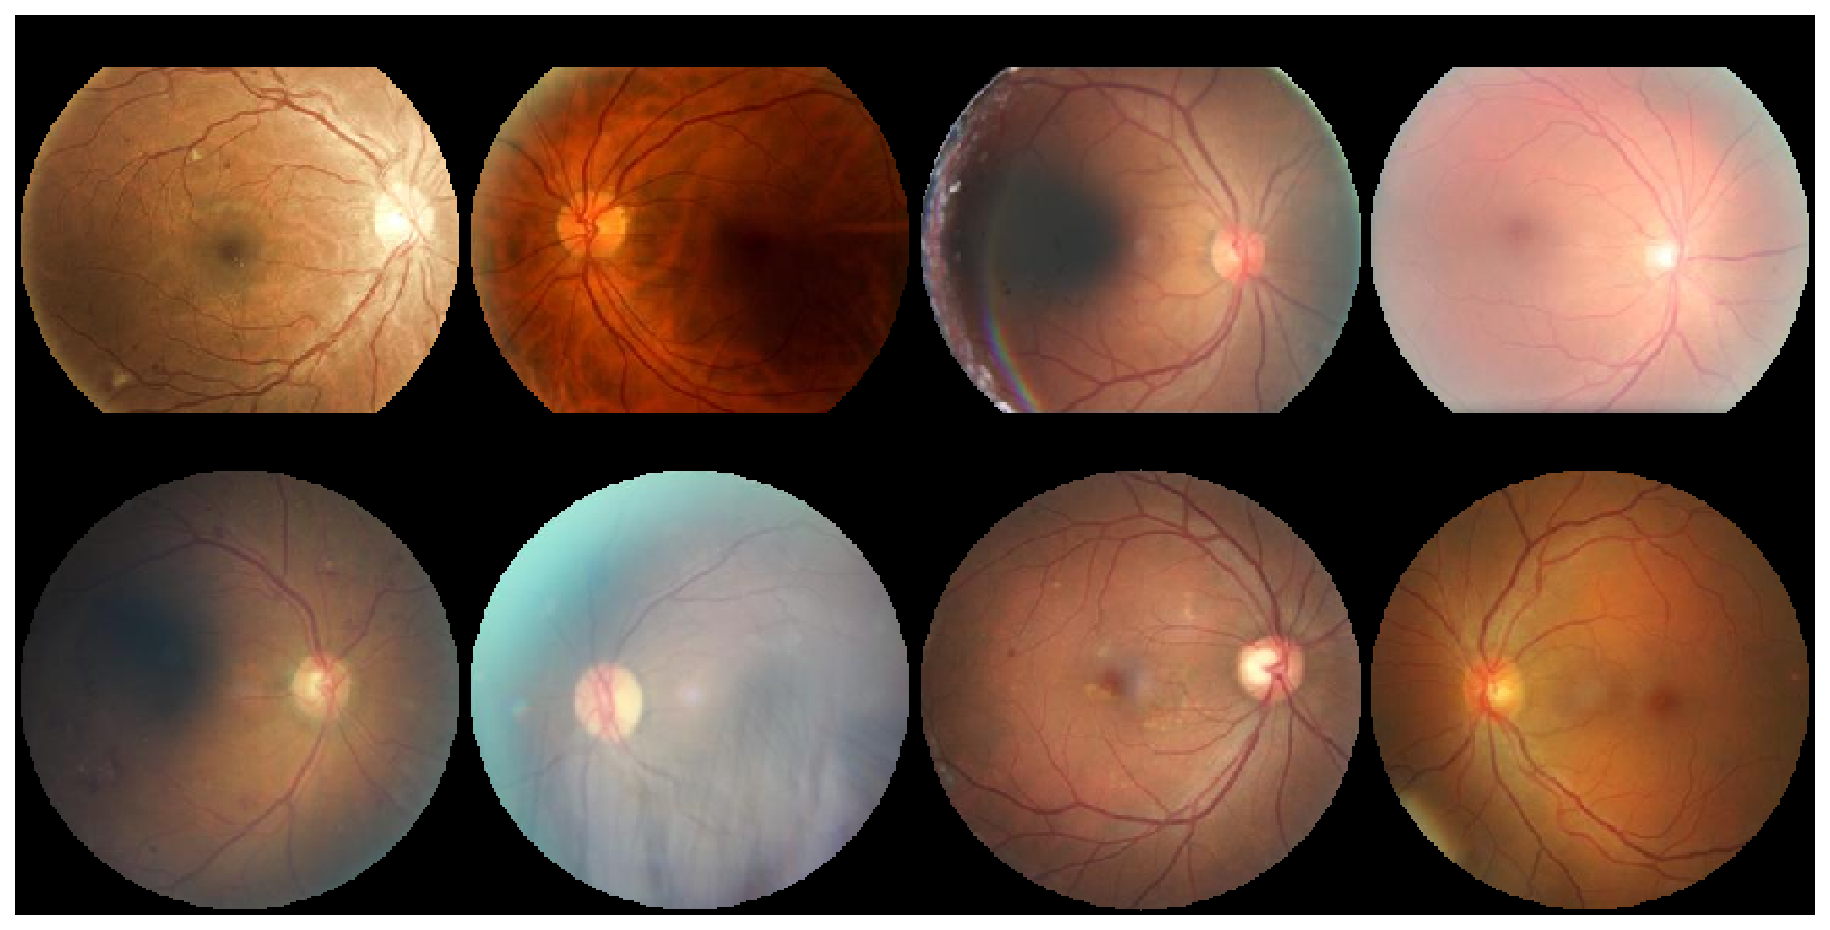
\includegraphics[width=1\linewidth]{stable.pdf} \caption{Εφαρμογή μασκών στο σύνολο δεδομένων Kaggle}
\label{figure:stable}  
\end{figure}

\subsection{Αλλαγή Δομής InceptionV3 με Χρήση Ασπρόμαυρης Μάσκας}
\label{subsec:5.4.5}

Στις εικόνες που δίνονται ως είσοδο στο νευρωνικό, όλη η πληροφορία του προβλήματος περιέχεται στον αμφιβληστροειδή ενώ το εξωτερικό φόντο δεν παρέχει καμία πληροφορία. Βάση αυτής της σκέψης πραγματοποιήθηκε μία μετατροπή στο νευρωνικού Inception V3. Η μετατροπή αυτή περιείχε  τον πολλαπλασιασμό των χαρτών χαρακτηριστικών με μία ασπρόμαυρη μάσκα με μηδενισμένα τα εικονοστοιχεία του φόντο και με τιμή ένα στα εικονοστοιχεία στην περιοχή του αμφιβληστροειδούς. Παρακάτω θα δοθούν κάποιες επιπλέον λεπτομέρειες για τη μέθοδο.

Έγινε χρήση εικόνων τεσσάρων καναλιών αντί τριών. Τα τρία  κανάλια περιείχαν την rgb εικόνα ενώ στο τέταρτο τοποθετήθηκε μία ασπρόμαυρη μάσκα. Έγινε χρήση 2 ειδών μάσκας: η μία μάσκα περιείχε ολόκληρο τον αμφιβληστροειδή ενώ η δεύτερη είχε κομμένο το πάνω και κάτω μέρος κατά αναλογία με τις εικόνες του συνόλου δεδομένων Kaggle.  Καθώς το Keras περιορίζει τον τύπο δεδομένων και τον αριθμό καναλιών που μπορεί να δεχτεί ως είσοδο το εκάστοτε νευρωνικό δίκτυο, για να είναι δυνατή η αποθήκευση πληροφορίας σε τέσσερα κανάλια έγινε χρήση rgba εικόνων. Οι  rgba εικόνες περιέχουν στο τρία πρώτα κανάλια τις εικόνες rgb και στο τέταρτο κανάλι τις τιμές που καθορίζουν την αδιαφάνεια ενός χρώματος, 0 (πλήρως διαφανές) και 1.0 (πλήρως αδιαφανές). Ένα δείγμα των εικόνων που δημιουργήθηκαν παρουσιάζονται στη εικόνα \ref{figure:rgba}. Να σημειωθεί ότι η χρήση εικόνων rgba έγινε για πρακτικούς λόγους καθώς έπρεπε να βρεθεί τρόπος να δοθούν ως είσοδο στο νευρωνικό εικόνες με τέσσερα κανάλια.

\begin{figure}[!h]
\centering
\begin{subfigure}{.5\textwidth}
  \centering
  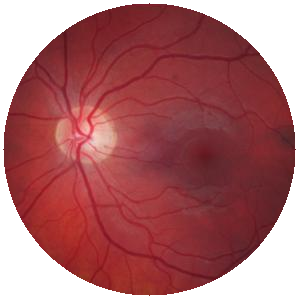
\includegraphics[scale=0.5]{rgba.png}
  \caption{Δείγμα 1}
  \label{fig:rgba1}
\end{subfigure}
\qquad
\begin{subfigure}{.5\textwidth}
  \centering
  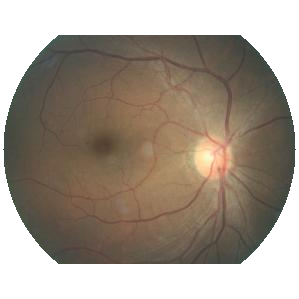
\includegraphics[scale=0.5]{rgb2.png}
  \caption{Δείγμα 2}
  \label{fig:rgba2}
\end{subfigure}
\caption{Παραδείγματα RGBA εικόνων}
\label{figure:rgba}
\end{figure}

Το τέταρτο κανάλι χρησιμοποιήθηκε ως μάσκα στους παραγόμενους χάρτες χαρακτηριστικών. Ουσιαστικά μετά από κάθε συνελικτικό επίπεδο, μέχρι τη μείωση σε 8x8 χάρτες χαρακτηριστικών, εφαρμόζονταν πολλαπλασιασμός κάθε χάρτη χαρακτηριστικών με τη μάσκα. Για να είναι δυνατός ο πολλαπλασιασμός οι διαστάσεις της αρχικής μάσκας μειωνώταν ανάλογα με τις διαστάσεις των χαρτών χαρακτηριστικών. 

Γενικά, το νευρωνικό Inception V3 περιέχει συνεχή μείωση των διαστάσεων των χαρτών χαρακτηριστικών με παράλληλη αύξηση των καναλιών τους, το οποίο υλοποιείται με συνελικτικά επίπεδα και επίπεδα υποδειγματοληψίας. Στα τελευταία επίπεδα παράγονται 17x17 χάρτες χαρακτηριστικών και στη συνέχεια γίνεται η τελική μείωση σε 8x8 χάρτες χαρακτηριστικών. Αποφασίστηκε η μη χρήση μάσκας στους 8x8 χάρτες χαρακτηριστικων καθώς οι διαστάσεις ήταν πολύ μικρές και θα μπορούσε να χαθεί χρήσιμη πληροφορία στα άκρα.



Για να γίνουν τα παραπάνω καθώς το Inception V3 του Keras καλείται σαν συνάρτηση και δεν επιδέχεται αλλαγές στη δομή του, ο κώδικας του Inception V3 κατέβηκε τοπικά και μετά από κάποιες αλλαγές ήταν δυνατή η χρήση του ως τοπική συνάρτηση τους συστήματος. Στη συνέχεια προστέθηκαν όλες οι αλλαγές που περιγράφηκαν παραπάνω και το σύστημα ήταν έτοιμο να τρέξει. Το σύστημα δεν παρουσίασε βελτιωμένα αποτελέσματα. Στην εικόνα \ref{figure:masked} παρουσιάζονται κάποιοι χάρτες χαρακτηριστικών μετά την εφαρμογή της μάσκας. Όπως είναι φανερό το φόντο δεν έχει καμία ενεργοποιημένη περιοχή.

\begin{figure}[!h]
    \centering
      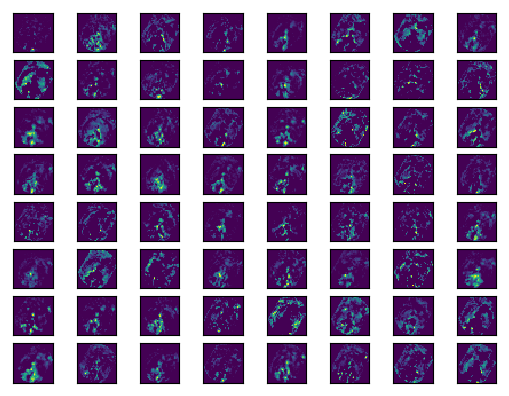
\includegraphics[width=0.8\linewidth]{FMmask.png} \caption{Χάρτες χαρακτηριστικών μετά την εφαρμογή μάσκας}
\label{figure:masked}  
\end{figure}



